\ifx\atempxetex\usewhat
\XeTeXinputencoding "utf-8"
\fi
\defaultfont

 \chapter{高级文件I/O}

在第二章,我们介绍了Linux下基本的 I/O 系统调用。这些调用不仅是文件I/O的基础,也是Linux下所有通信方式的基础。在第三章,我们了解到在基础I/O系统调用之上经常需要在用户空间做缓冲,并学习了一个用户空间缓冲的解决方案,即C的标准I/O库。在本章,我们将看到Linux提供的更多高级 I/O 系统调用:

\begin{eqlist*}
\item[\emph{散布/聚集 I/O}] I/O允许在单次调用中同时对多个缓冲区做读取或者写入操作,适合于聚集多个不同数据结构进行统一的I/O操作。
\item[\emph{epoll}] poll()和select()的改进版,在一个程序需要处理数百个文件描述符的时候很有用。
\item[\emph{内存映射I/O}] 将文件映射到内存,可以通过简单的内存管理方式来处理文件;适合有特殊要求的I/O。
\item[\emph{文件I/O提示}] 允许进程将文件I/O使用上的一些提示信息提供给内核; 能提升 I/O 性能。
\item[\emph{异步I/O}] 允许进程发出多个I/O请求而且不必等待其完成; 适用于不使用线程的情况下处理重负载I/O操作。
\end{eqlist*}

本章结束部分将讨论性能问题和内核的 I/O 子系统。

\section{散布/聚集 I/O}

散布聚集I/O是一种可以在单次系统调用中操作多个缓冲区的I/O方法,可以将单个数据流的内容写到多个缓冲区,或者把单个数据流读到多个缓冲区中。这样命名是因为数据被散布到一个缓冲区向量,或者从一个缓冲区向量聚集。这种方法的另一个名字是向量I/O。相对的,第二章提到的标准读写系统调用可以称作线性I/O。

散布/聚集 I/O与线性I/O相比有如下几个优点:

\begin{eqlist*}
\item[\emph{更自然的处理方式}] 如果你的数据是分段的(例如预处理过的头文件字段)向量I/O提供了直观的处理方式。
\item[\emph{效率}] 单个向量I/O操作能代替多个线性I/O操作。
\item[\emph{性能}] 除了系统调用次数的降低,由于内部优化,向量I/O比线性I/O提供更好的性能。
\item[\emph{原子性}] 不同于多个线性I/O操作,一个进程可以执行单个向量I/O操作而且避免了与其它进程交叉操作的风险。
\end{eqlist*}

我们也可以不使用散布/聚集 I/O机制,使用更自然的I/O方法,保证操作原子性。一个进程可以在写之前把分散的向量写到一个缓冲区中,也可以在读之后,把接受到的数据分散到多个缓冲区向量中,即手工实现用户空间的散布和聚集。但是这样处理是低效和无趣的。

\subsection{readv()和writev()}

Linux实现了POSIX 1003.1-2001中定义的两个使用散布/聚集机制的系统调用。Linux实现了上节所述的所有特性。

readv()从fd读取count个segment到iov描述的缓冲区中\footnote[1]{译者注:此处的segment指一个iov结构体}:

\begin{lstlisting}
  #include <sys/uio.h>
  ssize_t readv (int fd, const struct iovec *iov, int count);
\end{lstlisting}

writev()从iov描述的缓冲区中读取count个segment的数据并写入fd中:

\begin{lstlisting}
  #include <sys/uio.h>
  ssize_t writev (int fd, const struct iovec *iov, int count);
\end{lstlisting}

除了操作多个缓冲区外,readv()和writev()的行为和read(),write()一样。

每个iovec结构体描述一个独立的缓冲区,我们称其为\emph{段(segment)}:

\begin{lstlisting}
  #include <sys/uio.h>
  struct iovec {
    void *iov_base;
    size_t iov_len;
  };
\end{lstlisting}

一组segment的集合称为向量(vector)。每个段描述了所要读写的缓冲区的地址和长度。readv()在处理下个缓冲区之前会填满当前缓冲区的iov\_len 个字节。 writev()在处理下个缓冲区之前,把当前缓冲区所有iov\_len个字节数据输出。两个函数从iov[0]到iov[1],直到iov[count-1]来顺序处理这些段。

\subsubsection{返回值}

操作成功时,readv()和writev()分别返回读写的字节数。返回值应该等于所有iov\_len的和。出错时,返回-1,并且设置errno。这些系统调用可能会返回任何read()和write()可能返回的错误,遇到相同错误时,errno会设置为同样的值。此外,标准定义了两种额外的错误。

第一种情况,返回值类型是ssize\_t,如果iov\_len的和大于SSIZE\_MAX,则不做处理,返回-1,errno设置为EINVAL。

第二种情况,POSIX 声明count必须大于0,小于等于IOV\_MAX(在\\<limits.h>中定义)。在Linux中,IOV\_MAX通常是1024。如果count为0,系统调用返回0。\footnote[2]{注意,在其他的Unix中,当count为0时,可能将errno设置为EINVAL。这在标准中是明确规定的,如果count为0,可以设置为EINVAL或者由系统做专门处理。}如果count大于IOV\_MAX,不做处理,返回-1,errno设置为\\EINVAL。

\begin{center}
\begin{boxedminipage}{\textwidth}
\parindent=2em
\begin{center}\textbf{优化count}\end{center}

在向量 I/O 操作中,内核必须申请内核数据结构来表示每个段(segment)。通常,申请是基于count的大小动态进行的。出于优化的目的,如果count足够小的话,内核会在栈上创建几个段,通过避免动态分配内存,来获得性能上的一些提升。这个阈值一般为8,所以如果count小于等于8时,向量I/O操作会以一种高效的内存使用方式运行。

在大多数情况下,你不知道一次向量I/O需要传递多少段。当你犹豫是否试用一个很小的值时,选择8或更小的值肯定会得到性能的提升。
\end{boxedminipage}
\end{center}

\subsubsection{writev()示例}

让我们看一个简单的例子,把一个含有3个段,且每个段包含不同长度的字符串的向量写入一个缓冲区。这个程序足以演示writev()的功能,同时也可以作为一段有用的代码片段:

\begin{lstlisting}
  #include <stdio.h>
  #include <sys/types.h>
  #include <sys/stat.h>
  #include <fcntl.h>
  #include <string.h>
  #include <sys/uio.h>
  int main ()
  {
    struct iovec iov[3];
    ssize_t nr;
    int fd, i;
    char *buf[] = {"The term buccaneer comes from the word boucan.\n", "A boucan is a wooden frame used for cooking meat.\n", "Buccaneer is the West Indies name for a pirate.\n" };
    fd = open ("buccaneer.txt", O_WRONLY | O_CREAT | O_TRUNC);
    if (fd == -1) {
      perror ("open");
      return 1;
     }
     /* fill out three iovec structures */
     for (i = 0; i < 3; i++) {
       iov[i].iov_base = buf[i];
       iov[i].iov_len = strlen (buf[i]+1);
     }
     /* with a single call, write them all out */
     nr = writev (fd, iov, 3);
     if (nr == -1) {
       perror ("writev");
       return 1;
     }
     printf ("wrote %d bytes\n", nr);
     if (close (fd)) {
       perror ("close");
       return 1;
     }
     return 0;
  }
\end{lstlisting}

运行该程序,其结果如下:

\begin{verbatim}
  $ ./writev
  wrote 148 bytes
\end{verbatim}

读取该文件,内容如下:

\begin{verbatim}
  $ cat buccaneer.txt
  The term buccaneer comes from the word boucan.
  A boucan is a wooden frame used for cooking meat.
  Buccaneer is the West Indies name for a pirate.
\end{verbatim}

\subsubsection{readv()示例}

现在我们使用readv()来从前面生成的文本文件读取数据。这个程序同样也很简单:

\begin{lstlisting}
  #include <stdio.h>
  #include <sys/types.h>
  #include <sys/stat.h>
  #include <fcntl.h>
  #include <sys/uio.h>
  int main ()
  {
    char foo[48], bar[51], baz[49];
    struct iovec iov[3];
    ssize_t nr;
    int fd, i;
    fd = open ("buccaneer.txt", O_RDONLY);
    if (fd == -1) {
      perror ("open");
      return 1;
    }
    /* set up our iovec structures */
    iov[0].iov_base = foo;
    iov[0].iov_len = sizeof (foo);
    iov[1].iov_base = bar;
    iov[1].iov_len = sizeof (bar);
    iov[2].iov_base = baz;
    iov[2].iov_len = sizeof (baz);
    /* read into the structures with a single call */
    nr = readv (fd, iov, 3);
    if (nr == -1) {
      perror ("readv");
      return 1;
    }
    for (i = 0; i < 3; i++)
      printf ("%d: %s", i, (char *) iov[i].iov_base);
    if (close (fd)) {
      perror ("close");
      return 1;
    }
    return 0;
  } 
\end{lstlisting}

在运行上个程序之后,运行该程序产生了如下输出:

\begin{verbatim} 
  $ ./readv
  0: The term buccaneer comes from the word boucan.
  1: A boucan is a wooden frame used for cooking meat.
  2: Buccaneer is the West Indies name for a pirate.
\end{verbatim}

\subsubsection{实现}

我们可以在用户空间实现一个简单的readv()和writev(),类似的代码如下:

\begin{lstlisting}
  #include <unistd.h>
  #include <sys/uio.h>
  ssize_t naive_writev (int fd, const struct iovec *iov, int count)
  {
    ssize_t ret = 0;
    int i;
    for (i = 0; i < count; i++) {
      ssize_t nr;
      nr = write (fd, iov[i].iov_base, iov[i].iov_len);
      if (nr == -1) {
        ret = -1;
        break;
      }
      ret += nr; 
    }
    return ret;
  }
\end{lstlisting}

幸运的是,这不是Linux的实现:Linux下readv()和writev()作为系统调用实现,在内部使用散布/聚集 I/O。实际上,内核里的所有I/O都是向量I/O;read()和write()是只有一个向量的向量I/O,且向量中只有一个段。

\section{Event Poll接口}

由于poll()和select()的局限,2.6内核\footnote[1]{epoll在2.5.44开发版内核中加入,接口最终的完成在2.5.66}引入了event poll(epoll)机制。虽然比前两个实现复杂了很多,epoll解决了它们共有的基本性能问题,并增加了一些新的特性。

poll()和select()(见第二章)每次调用时都需要所有被监听的文件描述符。内核必须遍历所有被监视的文件描述符。当这个表变得很大时---包含上百,甚至上千个文件描述符时---每次调用时的遍历就成为了明显的瓶颈。

epoll把监听注册从实际监听中分离出来,从而解决了这个问题。一个系统调用初始化一个epoll上下文,另一个从上下文中加入或删除需要监视的文件描述符,第三个执行真正的事件等待(event wait)。

\subsection{创建一个新的epoll实例}

使用epoll create()创建一个epoll上下文:

\begin{lstlisting}
   #include <sys/epoll.h>
   int epoll_create (int size)
\end{lstlisting}

调用成功,epoll\_create()创建一个epoll实例,返回与该实例关联的文件描述符。这个文件描述符和真正的文件没有关系,仅仅是为了后续调用使用epoll而创建的。size参数告诉内核需要监听的文件描述符数目,但不是最大值。传递一个适当的近似值会带来性能的提升,但不需要给出确切的数字。出错时,返回-1,设置errno为下列值之一:

\begin{eqlist*}
\item[\textbf{EINVAL}] size 不是正数。
\item[\textbf{ENFILE}] 系统达到打开文件数的上限。
\item[\textbf{ENOMEN}] 没有足够的内存来完成该次操作。
\end{eqlist*}

一个标准的调用如下:

\begin{lstlisting}
  int epfd;
  epfd = epoll_create (100); /* plan to watch ~100 fds */
  if (epfd < 0)
    perror ("epoll_create");
\end{lstlisting}

epoll\_create()返回的文件描述符需要调用close()关闭。

\subsection{控制epoll}

epoll\_ctl()可以向指定的epoll上下文中加入或删除文件描述符:

\begin{lstlisting}
  #include <sys/epoll.h>
  int epoll_ctl (int epfd, int op, int fd, struct epoll_event *event);
\end{lstlisting}

头文件<sys/epoll.h>中定义了epoll event结构体:

\begin{lstlisting}
  struct epoll_event {
    __u32 events; /* events */
    union {
      void *ptr;
      int fd;
      __u32 u32;
      __u64 u64;
    } data;
  };
\end{lstlisting}

epoll ctl()成功调用将关联epoll实例和epfd。参数op指定对fd要进行的操作。event参数描述epoll更具体的行为。

以下是参数op的有效值:

\begin{eqlist*}
\item[\textbf{EPOLL\_CTL\_ADD}] 把fd指定的文件添加到epfd指定的epoll实例监听集中,监听event中定义的事件。
\item[\textbf{EPOLL\_CTL\_DEL}] 把fd指定的文件从epfd指定的epoll监听集中删除。
\item[\textbf{EPOLL\_CTL\_MOD}] 使用event改变在已有fd上的监听行为。
\end{eqlist*}

epoll events结构体中的events参数列出了在给定文件描述符上监听的事件。多个事件可以使用位或运算同时指定。以下为有效值:

\begin{eqlist*}
\item[\textbf{EPOLLERR}] 文件出错。即使没有设置,这个事件也是被监听的。
\item[\textbf{EPOLLET}] 在监听文件上开启边沿触发。(见下一部分''边沿触发和水平触发条件'')。默认行为是水平触发。
\item[\textbf{EPOLLHUP}] 文件被挂起。即使没有设置,这个事件也是被监听的。
\item[\textbf{EPOLLIN}] 文件未阻塞,可读。
\item[\textbf{EPOLLONESHOT}] 在一次事件产生并被处理之后,文件不再被监听。必须使用EPOLL\_CTL\_MOD指定新的事件,以便重新监听文件。
\item[\textbf{EPOLLOUT}] 文件未阻塞,可写。
\item[\textbf{EPOLLPRI}] 高优先级的带外数据可读。
\end{eqlist*}

event\_poll中的data字段由用户使用。确认监听事件后,data会被返回给用户。通常将event.data.fd为设定fd,这样就可以知道哪个文件描述符触发事件。

成功后,epoll\_ctl()返回0。失败返回-1,并设置errno为下列值:

\begin{eqlist*}
\item[\textbf{EBADF}] epfd不是一个有效epoll实例,或者fd不是有效文件描述符。
\item[\textbf{EEXIST}] op为EPOLL\_CTL\_ADD,但是fd已经与epfd关联。
\item[\textbf{EINVAL}] epfd不是一个epoll实例,epfd和fd相同,或者op无效。
\item[\textbf{ENOENT}] op是EPOLL\_CTL\_MOD,或者EPOLL\_CTL\_DEL,但是fd没有与epfd关联。
\item[\textbf{ENOMEN}] 没有足够内存完成进程的请求。
\item[\textbf{EPERM}] fd不支持epoll。
\end{eqlist*}

在epfd实例中加入一个fd指定的监听文件,可以使用如下代码:

\begin{lstlisting}
  struct epoll_event event;
  int ret;
  event.data.fd = fd; /* return the fd to us later */
  event.events = EPOLLIN | EPOLLOUT;
  ret = epoll_ctl (epfd, EPOLL_CTL_ADD, fd, &event);
  if (ret)
    perror ("epoll_ctl");
\end{lstlisting}

修改epfd实例中的fd上的一个监听事件,可以使用如下代码:

\begin{lstlisting}
  struct epoll_event event;
  int ret;
  event.data.fd = fd; /* return the fd to us   later */
  event.events = EPOLLIN;
  ret = epoll_ctl (epfd, EPOLL_CTL_MOD, fd,  &event);
  if (ret)
    perror ("epoll_ctl");
\end{lstlisting}
相反的,从epfd中移除在fd上的一个监听事件,可以使用如下代码:

\begin{lstlisting}
  struct epoll_event event;
  int ret;
  ret = epoll_ctl (epfd, EPOLL_CTL_DEL, fd, &event);
  if (ret)
    perror ("epoll_ctl");
\end{lstlisting}

需要注意的是,op为EPOLL\_CTL\_DEL时,因为没有设置事件掩码,event参数可以为NULL。2.6.9以前的内核中,会检查该参数是否为非空。为了兼容旧内核,必须传递一个有效的non-NULL指针;该指针不会被访,2.6.9版本修复了这个bug。
 
\subsection{等待Epoll事件}

epoll\_wait()等待给定epoll实例关联的文件描述符上的事件:

\begin{lstlisting}
  #include <sys/epoll.h>
  int epoll_wait (int epfd, struct epoll_event *events, int maxevents, int timeout);
\end{lstlisting}

对epoll\_wait()的调用等待epoll实例epfd中的文件fd上的事件,时限为timeout毫秒。成功返回,events指向包含epoll\_event结构体(该结构体描述了每个事件)的内存,且最多可以有maxevents个事件。返回值是事件数,出错返回 -1,并将errno设置为以下值:

\begin{eqlist*}
\item[\textbf{EBADF}] epfd是无效文件描述符。
\item[\textbf{EFAULT}] 进程对events指向的内存无写权限。
\item[\textbf{EINTR}] 系统调用在完成前被信号中断。
\item[\textbf{EINVAL}] epfd不是有效epoll实例,或者maxevents小于等于0。
\end{eqlist*}

如果timeout为0,即使没有事件发生,调用也立即返回,此时调用返回0。如果timeout为-1,调用将一直等待到有事件发生。

当调用返回,epoll\_event结构体中的events字段描述了发生的事件。data字段包含了所有用户在调用epoll\_ctl()前的设置。

一个完整的epoll\_wait()例子如下:

\begin{lstlisting}
  #define MAX_EVENTS    64
  struct epoll_event *events;
  int nr_events, i, epfd;
  events = malloc (sizeof (struct epoll_event) * MAX_EVENTS);
  if (!events) {
    perror ("malloc");
    return 1;
  }
  nr_events = epoll_wait (epfd, events, MAX_EVENTS, -1);
  if (nr_events < 0) {
    perror ("epoll_wait");
    free (events);
    return 1;
  }
  for (i = 0; i < nr_events; i++) {
    printf ("event=%ld on fd=%d\n", events[i].events, events[i].data.fd);
    /*
     * We now can, per events[i].events, operate on
     * events[i].data.fd without blocking.
     */
  }
  free (events);   
\end{lstlisting}

我们将在第八章学习malloc()和free()。

\subsection{边沿触发事件和水平触发事件}

如果epoll\_ctl()的参数event中的events项设置为EPOLLET,fd上的监听方式为边沿触发,相反的是水平触发。考虑下面的生产者和消费者在通过unix管道通信时的情况。

\begin{enumerate}
\item 生产者向管道写入1kb数据。
\item 消费者在管道上调用epoll\_wait(),等待pipe出现数据,从而可读。
\end{enumerate}

对于水平触发的监听,在步骤2里对epoll\_wait()的调用将立即返回,以表明pipe可读。对于边沿触发的监听,这个调用直到步骤1发生后才会返回。也就是说,即使调用epoll\_wait()时管道已经可读,调用仍然会等待直到有数据写入,之后返回。

水平触发是默认行为。也是poll()和select()的行为,也是大多数开发者所期望的。边沿触发需要一个不同的方式来写程序,通常利用非阻塞I/O,并需要仔细检查EAGAIN。

\begin{wrapfigure}{l}{2.5cm}
  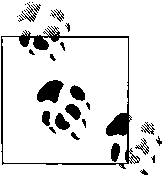
\includegraphics[width=2cm,clip]{paipai.png}
\end{wrapfigure}
\mbox{}该术语来自电气工程领域。水平触发在一个状态发生时触发。边沿触发只有在状态改变的时候才会产生。水平触发在只关心状态时有用。边沿触发则在关心事件本身时有用。
 
\section{存储映射}

除了标准文件I/O,内核提供了另一种I/O方式,允许应用程序将文件映射到内存中,即内存和文件中数据是一一对应的。程序员可以直接通过内存来访问文件,就像操作内存的数据块一样,甚至可以写入内存数据区,然后通过透明的映射机制将文件写入磁盘。

Linux实现了POSIX.1中定义的mmap()系统调用,该调用将对象映射到内存中。本节我们讨论mmap()在I/O中将文件映射到内存的功能;在第八章,我们将看到该调用的其它应用。

\subsection{mmap()}

mmap()调用请求内核将fd表示的文件中从offset处开始的len个字节数据映射到内存中。如果包含了addr,表明优先使用addr为内存中的开始地址。访存权限由prot指定,flags指定了其他的操作行为。

\begin{lstlisting}
  #include <sys/mman.h>
  void * mmap (void *addr, size_t len, int prot, int flags, int fd, off_t offset);
\end{lstlisting}

addr参数告诉内核映射文件的最佳地址。这仅仅是提示,而不是强制,大部分用户传递0。调用返回内存映射区域的开始地址。

prot参数描述了对内存区域所请求的访问权限。如果是PROT\_NONE,此时映射区域无法访问(没有意义),也可以是以下标志位的比特位的或运算值:

\begin{eqlist*}
\item[\textbf{PROT\_READ}] 页面可读。
\item[\textbf{PROT\_WRITE}] 页面可写。
\item[\textbf{PROT\_EXEC}] 页面可执行。
\end{eqlist*}

要求的访存权限不能和打开文件的访问模式冲突。举例来说,如果程序以只读方式打开文件,prot不能设置为PROT\_WRITE。

\begin{center}
\begin{boxedminipage}{\textwidth}
\parindent=2em
\begin{center}\textbf{保护标志,体系结构和安全性}\end{center}

POSIX定义了四种保护位(读,写,执行,避开),一些体系结构只支持其中的子集。其实这很正常,例如对于处理器来讲,读和执行没有区别。这种情况下,处理器可能只有一个读标志。在这些操作系统上,PROT\_READ即代表PROT\_EXEC。不久之前,x86还是这样的系统。

当然,依赖这样的处理方式会导致程序不可移植。可移植的程序在他们需要执行映射中的代码时,会相应的设置PROT\_EXEC。

从另一面来说,这是造成缓冲区溢出攻击盛行的原因之一,即使一个映射不允许执行操作,但处理器仍会执行映射中的代码。

最近x86处理器加入了NX(no-execute)位,它允许可读,但不可执行的映射。在较新的系统上,PROT\_READ不再等同于PROT\_EXEC。
\end{boxedminipage}
\end{center}

flag参数描述了映射的类型和一些行为。其值为以下值按按位或运算的值:

\begin{eqlist*}
\item[\textbf{MAP\_FIXED}] 告诉mmap()把addr看作强制性要求,而不是建议。如果内核无法映射文件到指定地址,调用失败。如果地址和长度指定的内存和已有映射有重叠区域,重叠区的原有内容被丢弃,然后被新内容填充。该选项需要深入了解进程的地址空间,不可移植,所以不鼓励使用。
\item[\textbf{MAP\_PRIVATE}] 映射区不共享。文件映射采用了写时拷贝,进程对内存的任何改变不影响真正的文件或者其它进程的映射。
\item[\textbf{MAP\_SHARED}] 和所有其它映射该文件的进程共享映射内存。对内存的写操作等效于写文件。读该映射区域会受到其他进程的写操作的影响。
\end{eqlist*}

MAP\_SHARED和MAP\_PRIVATE必须指定其中之一,但不能同时指定。更多的标志将在第8章讨论。

当你映射一个文件描述符的时候,描述符引用计数增加。因此,如果你映射文件后关闭文件,你的进程依然可以访问该文件。当你取消映射或者进程终止时,对应的文件引用计数会减 1。

下面的示例代码中以只读方式映射fd所指向的文件,从第一个字节开始,长度为len个字节:

\begin{lstlisting}
  void *p;
  p = mmap (0, len, PROT_READ, MAP_SHARED, fd, 0);
  if (p == MAP_FAILED)
    perror ("mmap");
\end{lstlisting}

图4-1 演示了mmap()的参数对文件与进程地址空间映射的影响。

\begin{figure}[htp]
 \centering
 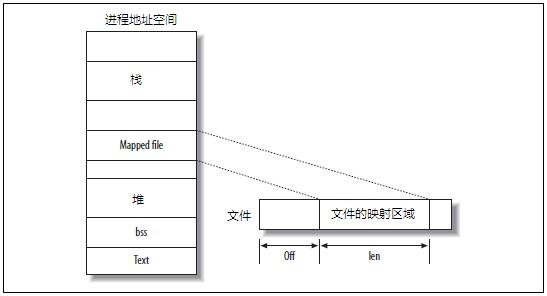
\includegraphics[width=\textwidth]{ch4.jpg}
 \caption{映射文件至进程地址空间}
\end{figure}

\subsubsection{页大小}

\emph{页}是内存中允许具有不同权限和行为的最小单元。因此,页是内存映射的基本块,同时也是进程地址空间的基本块。

mmap()调用操作页。addr和offset参数都必须按页大小对齐。也就是说,它们必须是页大小的整数倍。

所以,映射区域是整数倍个的页。如果len参数不能按页对齐(可能因为需要映射的文件大小不是页大小的整数倍)映射区域延伸到下个空页。多出来的内存,即最后一个有效字节和映射区域边界的区域,用0填充. 该区域的读操作都将返回0。即使使用MAP\_SHARED参数进行映射,写操作也不会影响文件。只有前len个字节需要写回文件。

\textbf{sysconf():}标准POSIX规定的获得页大小方法是通过sysconf(),它将返回一系列系统特定的信息:

\begin{lstlisting}
  #include <unistd.h>
  long sysconf (int name);
\end{lstlisting}

调用sysconf()返回name的值,如果name无效,返回-1。出错时,errno被设置为EINVAL。因为-1对一些情况来讲可能是有效值(例如limits,-1表示没有限制)。明智的做法是在调用前清空errno,并在调用后检查其值。

POSIX定义了\_SC\_PAGESIZE(SC\_PAGE\_SIZE与其同义),大小为一个页面的字节大小。因此,很容易获得页大小:

\begin{lstlisting}
  long page_size = sysconf (_SC_PAGESIZE);
\end{lstlisting}

\textbf{getpagesize():}Linux也提供了getpagesize()函数来获得页大小:

\begin{lstlisting}
  #include <unistd.h>
  int getpagesize (void);
\end{lstlisting}

调用getpagesize()将返回页按字节计数的大小。使用也比sysconf()简单:

\begin{lstlisting}
  int page_size = getpagesize ( );
\end{lstlisting}

并不是所有unix系统支持这个函数,POSIX 1003.1-2001弃用了该函数,在这里包含只是出于完整性考虑。

\textbf{页大小:}页大小由<asm/pages.h>中的宏PAGE\_SIZE定义。因此,第三种获得页大小的方法是:

\begin{lstlisting}
  int page_size= PAGE_SIZE ;
\end{lstlisting}

不同于前两种方法,这种方法是编译时获得页大小,而不是运行时。一些体系结构支持多种机型使用不同页大小,某些机型甚至支持多个不同的页大小。一个二进制文件应该能在给定体系结构下的所有机型上运行,即一次编译,到处运行。硬编码页大小则会终结这种可能性. 因此,你应该在运行时确定页的大小。因为addr和offset通常为0,这种设置并不困难。

此外,未来的内核可能不会将该宏导出到用户空间。我们在此提到它是因为在它在Unix代码中使用很频繁,但是不要在你自己程序中使用它。目前看来,sysconf()是最好的选择。

\subsubsection{返回值和错误码}

调用成功,mmap()返回映射区的地址。失败时,返回MAP\_FAILED,并设置相应的errno。mmap()从不返回0。

可能的errno值:

\begin{eqlist*}
\item[\textbf{EACESS}] 给定的文件描述符不是普通文件,或者打开模式和prot或者flags冲突。
\item[\textbf{EAGAIN}] 文件已被文件锁锁定。
\item[\textbf{EBADF}] 给定文件描述符无效。
\item[\textbf{EINVAL}] addr,len,off中的一个或多个无效。
\item[\textbf{ENFILE}] 打开文件数达到系统上限。
\item[\textbf{ENODEV}] 文件所在的文件系统不支持存储映射。
\item[\textbf{ENOMEM}] 没有足够的内存。
\item[\textbf{EOVERFLOW}] addr + len的结果超过了地址空间大小。
\item[\textbf{EPERM}] 设定了PROT\_EXEC,但是文件系统以不可执行方式挂载。
\end{eqlist*}

\subsubsection{相关信号}

两个和映射区域相关的信号:

\begin{eqlist*}
\item[\textbf{SIGBUS}] 当进程试图访问一块已经无效的映射区域时,该信号产生。比如,文件在映射后被截短。
\item[\textbf{SIGSEGV}] 当进程试图写一块只读的映射区域时,该信号产生。
\end{eqlist*}

\subsection{munmap()}

Linux提供了munmap()来取消mmap()的映射。

\begin{lstlisting}
  #include <sys/mman.h>
  int munmap (void *addr, size_t len);
\end{lstlisting}

munmap()移除进程地址空间从addr开始,len字节长的内存中的所有页面的映射。当映射被解除时,之前关联的内存区域不再有效,如果试图访问将产生SIGSEGV信号。

通常,munmap()的参数是上次mmap()调用的返回值和其参数len。

调用成功返回0;失败返回-1,errno被设置为相应的值。唯一标准的errno值为EINVAL,表明一个或多个参数无效。

作为实例,下面一段代码解除了内存中[addr, addr + len]区间内所有页的映射。

\begin{lstlisting}
  if (munmap (addr, len) == -1)
    perror ("munmap");
\end{lstlisting}

\subsection{存储映射例子}

我们来看一个例子,使用mmap将用户选择的文件输出到标准输出:

\begin{lstlisting}
  #include   <stdio.h>
  #include   <sys/types.h>
  #include   <sys/stat.h>
  #include   <fcntl.h>
  #include   <unistd.h>
  #include   <sys/mman.h>
  int main (int argc, char *argv[])
  {
    struct stat sb;
    off_t len;
    char *p;
    int fd;
    if (argc < 2) {
      fprintf (stderr, "usage: %s <file>\n", argv[0]);
      return 1;
     }
     fd = open (argv[1], O_RDONLY);
     if (fd == -1) {
       perror ("open");
       return 1;
     }
     if (fstat (fd, &sb) == -1) {
       perror ("fstat");
       return 1;           
     }
     if (!S_ISREG (sb.st_mode)) {
       fprintf (stderr, "%s is not a file\n", argv[1]);
       return 1;
     }
     p = mmap (0, sb.st_size, PROT_READ, MAP_SHARED, fd, 0);
     if (p == MAP_FAILED) {
       perror ("mmap");
       return 1;
     }
     if (close (fd) == -1) {
       perror ("close");
       return 1;
     }
     for (len = 0; len < sb.st_size; len++)
       putchar (p[len]);
     if (munmap (p, sb.st_size) == -1) {
       perror ("munmap");
       return 1;
     }
     return 0;
  }
\end{lstlisting}

在本例中,大家唯一不熟悉的系统调用为fstat(),我们将在第七章讲到。在这里,你仅仅需要知道fstat()返回给定文件的信息。S\_ISREG()宏可以检查这些信息,这样我们可以在映射前确保给定文件是个普通文件(相对于设备文件和目录而言)。映射一个非普通文件的行为取决于文件所在设备。一些设备是可以映射的,而有些是不可以的,映射会设置errno为EACCESS。

例子的剩余部分都是很直观的,传递一个文件名作为程序参数。打开文件,确保其为普通文件,映射,关闭,按字节打印文件到标准输出,最后取消映射。

\subsection{mmap()的优点}

相对于read(),write(),使用mmap()处理文件有很多优点。其中包括:

\begin{itemize}
\item 使用read()或write()系统调用需要从用户缓冲区进行数据读写,而使用映射文件进行操作,可以避免多余的数据拷贝。
\item 除了潜在的页错误,读写映射文件不会带来系统调用和上下文切换的开销。就像直接操作内存一样简单。
\item 当多个进程映射同一个对象到内存中,数据在进程间共享。只读和写共享的映射在全体中都是共享的;私有可写的尚未进行写时拷贝的页是共享的。
\item 在映射对象中搜索只需要一般的指针操作。而不必使用lseek()。
\end{itemize}

基于以上理由,mmap()是很多应用的明智选择。

\subsection{mmap()的缺陷}

使用mmap()时需要注意以下几点:

\begin{itemize}
\item 映射区域的大小通常是页大小的整数倍。因此,映射文件大小与页大小的整数倍之间有空间浪费。对于小文件,较大比重的空间被浪费。例如对于4kb的页,一个7字节的映射浪费了4089字节。
\item 存储映射区域必须在进程地址空间内。对于32位的地址空间,大量的大小各异的映射会导致大量的碎片出现,使得很难找到连续的大片空内存。这个问题在64位地址空间明显减少。
\item 创建和维护映射以及相关的内核数据结构有一定的开销。通过上节提到的消除读写时的不必要拷贝的,这些开销可以忽略,对于大文件和频繁访问的文件更是如此。
\end{itemize}

基于以上理由,处理大文件(浪费的空间只占很小的比重),或者在文件大小恰好被page大小整除时(没有空间浪费)优势很明显。

\subsection{调整映射的大小}

Linux提供了mremap()来扩大或减少已有映射的大小。这个函数是Linux特有的:

\begin{lstlisting}
  #define _GNU_SOURCE
  #include <unistd.h>
  #include <sys/mman.h>
  void * mremap (void *addr, size_t old_size, size_t new_size, unsigned long flags);
\end{lstlisting}

mremap()将映射区域[addr, addr + old size)的大小增加或减少到new\_size。依赖进程地址空间的可用大小和flags,内核可以同时移动映射区域。

\begin{wrapfigure}{l}{2.5cm}
  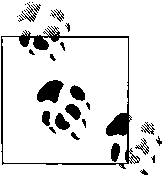
\includegraphics[width=2cm,clip]{paipai.png}
\end{wrapfigure}
\mbox{}[表示区域从低地址开始,包括低地址。)表示区域在高地址为止,不包括高地址,这个惯例称作间隔符号(interval notation)。

flags参数的值可以是0或者MREMAP\_MAYMOVE ,这意味在为了执行调整指定的大小,内核可以根据需求移动映射区域。如果内核可以移动映射,一个较大规模的大小调整操作就可能成功。

\subsubsection{返回值和错误码}

调用成功,mremap()返回指向新映射区域的指针。失败则返回MAP\_FAILED,设置errno为以下值:

\begin{eqlist*}
\item[\textbf{EAGAIN}] 内存区域被锁,不能调整大小。
\item[\textbf{EFAULT}] 给定范围内的一些页不是进程地址空间内的有效页,或者在重新映射给定页时出现问题。
\item[\textbf{EINVAL}] 一个参数无效。
\item[\textbf{ENOMEM}] 给定范围如果不进行移动则无法扩展(MREMAP\_MAYMOVE没有设置),或者进程地址空间内没有足够空闲空间。
\end{eqlist*}

glibc等库经常使用mremap()实现高效的realloc(),可以通过它调整一块由malloc()分配的内存。例如:

\begin{lstlisting}
  void * realloc (void *addr, size_t len)
  {
    size_t old_size = look_up_mapping_size (addr);
    void *p;
    p = mremap (addr, old_size, len, MREMAP_MAYMOVE);
    if (p == MAP_FAILED)
      return NULL;
    return p;
  }
\end{lstlisting}

这段代码只在所有malloc()操作是唯一的匿名映射时有效;即使如此,这段代码也能作为展示尽量提高性能的有用样例。这个例子假设程序员已经写了一个look\_up\_mapping\_size()函数。GNU C library使用mmap()及其相关函数来进行内存分配。我们将在第八章更深入的讨论这个话题。

\subsection{改变映射区域的权限}

POSIX定义了mprotect(),允许程序改变已有内存区域的权限:

\begin{lstlisting}
  #include <sys/mman.h>
  int mprotect (const void *addr, size_t len, int prot);
\end{lstlisting}

调用mprotect()会改变[addr, addr + len)区域内页的访问权限,addr是页对齐的。prot参数和mmap()的prot参数有同样的值:PROT\_NONE,PROT\_READ,PROT\_WRITE,PROT\_EXEC。这些值不是累积的;如果一块区域可读prot值设置了PROT\_WRITE,调用后该区域为只写。

在一些系统上,mprotect()只能操作之前由mmap()创建的区域。在Linux下,mprotect()可以操作任意区域的内存。

\subsubsection{返回值和错误码}

调用成功,mprotect()返回0。失败,返回-1,设置errno值为如下之一:

\begin{eqlist*}
\item[\textbf{EACCESS}] 内存不能设置prot所请求的权限。例如,你试图将一个只读打开的文件的映射设置为可写。
\item[\textbf{EINVAL}] addr无效或者没有页对齐。
\item[\textbf{ENOMEM}] 内核没有足够空间满足请求,或者请求区域内有页面不是进程地址空间内的有效部分。
\end{eqlist*}

\subsection{使用映射机制同步文件}

POSIX提供了一个使用存储映射机制并与fsync()等价的系统调用:

\begin{lstlisting}
  #include <sys/mman.h>
  int msync (void *addr, size_t len, int flags);
\end{lstlisting}

调用msync()可以将mmap()生成的映射在内存中的任何修改回写到磁盘,达到同步内存中的映射和被映射的文件的目的。具体来说,文件或者文件子集在内存中的映射从addr开始的len长度字节被写回到磁盘。addr参数必须是页对齐的,通常是上次mmap()调用的返回值。

不调用 msync(),无法保证在映射取消前,修改过的映射会被写回到硬盘。这一点与write()有所不同,被write()修改的缓冲区被保存在一个队列中等待被写回。当写入内存映射时,进程直接修改内核页缓存中的文件页,而无需经过内核。内核不会立刻同步页缓存到硬盘。

flag 参数控制同步操作的行为。它的值为以下值的按位或操作:

\begin{eqlist*}
\item[\textbf{MS\_ASYNC}] 指定同步操作异步发生。更新操作由系统调度,msync()会立即返回,不用等待write()操作完成。
\item[\textbf{MS\_INVALIDATE}] 指定该块映射的其它所有拷贝都将失效。未来对该文件任意映射的操作将直接同步到磁盘。
\item[\textbf{MS\_SYNC}] 指定同步操作必须同步进行。msync() 直到所有页写回磁盘后返回。
\end{eqlist*}

MS\_ASYNC和MS\_SYNC必须指定其一,二者不能共用。

用法很简单:

\begin{lstlisting}
  if (msync (addr, len, MS_ASYNC) == -1)
    perror ("msync");
\end{lstlisting}

这个例子是异步的将文件的映射区域[addr, addr+len)同步到磁盘。

\subsubsection{返回值和错误码}

调用成功,msync()返回0。失败,调用返回-1,设置errno为相应值。以下为errno的有效值:

\begin{eqlist*}
\item[\textbf{EINVAL}] flags 参数同时设置了MS\_SYNC和MS\_ASYNC,设置了除以上三个合法参数外的其他参数,或者没有页对齐。
\item[\textbf{ENOMEM}] 指定的内存区域(或其中一部分)没有被映射。注意按POSIX规定,Linux在请求同步一块部分解除映射的内存时,将返回ENOMEM,但是这样可能同步一些无效的区域。
\end{eqlist*}

在2.4.29版本的内核之前,msync()返回EFAULT,而不是ENOMEM。

\subsection{映射提示}

Linux提供了madvise()系统调用,可以让进程在如何访问映射区域上给内核一定的提示。内核会据此优化自己的行为,尽量更好的利用映射区域。内核一般会动态调整自己的行为,通常即便在没有明确提示时也能保证较好的性能,但是适当的提示信息可以确保在一定负载下获得所需的缓存和执行正确的预读。

调用会指示内核该如何对起始地址为addr,长度为len的内存映射区域进行操作。

\begin{lstlisting}
  #include <sys/mman.h>
  int madvise (void *addr, size_t len, int advice);
\end{lstlisting}

如果len为0,内核将对所有起始地址为addr的映射使用该提示信息。参数advice可以是下列之一:

\begin{eqlist*}
\item[\textbf{MADV\_NORMAL}] 对给定的内存区域,应用程序没有特殊提示,按正常方式操作。
\item[\textbf{MADV\_RANDOM}] 应用程序将以随机顺序访问指定范围的页。
\item[\textbf{MADV\_SEQUENTIAL}] 应用程序意图从低地址到高地址顺序访问指定范围的页。
\item[\textbf{MADV\_WILLNEED}] 应用程序将很快访问指定范围的页。
\item[\textbf{MADV\_DONTNEED}] 应用程序短期内不会访问指定范围内的页。
\end{eqlist*}

内核得到提示后真正采取的行为是与具体的实现相关的:POSIX仅仅指定了提示的含义,而没有规定具体的行为。2.6内核以如下方式进行处理:

\begin{eqlist*}
\item[\textbf{MADV\_NORMAL}] 内核行为照常,进行一定程度的预读。 
\item[\textbf{MADV\_RANDOM}] 内核不做预读,每次物理读操作只读取最小量的数据。
\item[\textbf{MADV\_SEQUENTIAL}] 内核大量预读。
\item[\textbf{MADV\_WILLNEED}] 内核将给定的页预读至内存。
\item[\textbf{MADV\_DONTNEED}] 内核释放所有和给定页相关的资源,丢弃所有被修改的,未同步写回的页。后续对映射数据访问会使数据重新载入内存。
\end{eqlist*}

典型用法如下:

\begin{lstlisting}
  int ret;
  ret = madvise (addr, len, MADV_SEQUENTIAL);
  if (ret < 0)
    perror ("madvise");
\end{lstlisting}

该调用告诉内核,进程意图连续访问内存区域[addr, addr + len)。

\begin{center}
\begin{boxedminipage}{\textwidth}
\parindent=2em
\begin{center}\textbf{预读}\end{center}

当Linux内核访问磁盘上的文件时,通常会采用众所周知的预读(readahead)来优化自己的操作。也就是说,当文件的某块内容被加载时,内核也会读取这块内容之后的块。如果随后有对该块的访问请求(例如连续访问某个文件时)内核可以马上返回数据。因为磁盘有缓冲区(磁盘自己也会有预读行为),而且文件通常是连续分布在磁盘的,这个优化的开销是很低的。

预读通常是有好处的,但是具体的优化效果依赖于预读的程度。很大的预读窗口在连续访问文件时很有效,而对随机访问来讲,预读则是无用的开销。

正如我们在第二章的“内核内幕”一节所讨论的,内核会动态的调整预读窗口,以保证在预读窗口中一定的命中率。高命中率则意味着最好使用再大一点的预读窗口,反之则提示使用小一点的预读窗口。应用程序可以通过madvise()系统调用来影响预读窗口的大小。
\end{boxedminipage}
\end{center}

\subsubsection{返回值和错误码}

调用成功,madvise()返回0,失败时,返回-1,设置errno为相应值。以下为有效错误值:

\begin{eqlist*}
\item[\textbf{EAGAIN}] 内核内部资源(可能是内存)不可用,进程可以重试。
\item[\textbf{EBADF}] 区域存在,但是没有映射到文件。
\item[\textbf{EINVAL}] 参数len是负的,addr不是页对齐的,advice参数无效,或者页面被锁,或以MADV\_DONTNEED方式共享该区域.
\item[\textbf{EIO}] 使用MADV\_WILLNEED操作时引起的内部I/O错误。
\item[\textbf{ENOMEM}] 给定的区域不是进程地址空间的有效映射,或者设置MADV\_WILLNEED,但是没有足够内存可供分配。
\end{eqlist*}

\section{普通文件I/O提示}

上一小节,我们学习了如何给内核提供存储映射的操作提示。在本节,我们将学习在普通文件I/O 时,如何给内核提供操作提示。Linux提供了两个满足要求的函数:posix\_fadvise()和readahead()。

\subsection{posix\_fadvise()}

正如它的名字一样,该函数由POSIX 1003.1-2003定义:

\begin{lstlisting}
  #include <fcntl.h>
  int posix_fadvise (int fd, off_t offset, off_t len, int advice);
\end{lstlisting}

调用posix\_fadvise()会给出内核在文件fd的[offset, offset + len) 范围内操作提示。如果len为0,则该提示作用于区间[offset, length of file]。一般用法是设置len和offset为0,从而使设置应用到整个文件。

advice 的可用选项和madvise()类似。准确的讲,是以下选项的其中之一:

\begin{eqlist*}
\item[\textbf{POSIXFADV\_NORMAL}] 应用程序在给定文件的给定区域没有特殊要求,按正常情况处理。
\item[\textbf{POSIX\_FADV\_RANDOM}] 应用程序在给定范围内趋向于随机访问。
\item[\textbf{POSIX\_FADV\_SEQUENTIAL}] 应用程序在给定范围内趋向于从低地址到高地址顺序访问。
\item[\textbf{POSIX\_FADV\_WILLNEED}] 应用程序可能在最近访问指定范围。
\item[\textbf{POSIX\_FADV\_NOREUSE}] 应用程序可能在最近访问给定范围,但只访问一次。
\item[\textbf{POSIX\_FADV\_DONTNEED}] 应用程序最近可能不会访问给定范围。
\end{eqlist*}

和madvise()一样,内核对这些提示的处理因不同的实现而有所区别,甚至不同版本的Linux内核的处理方式也不尽相同。下面是目前内核的处理方式:

\begin{eqlist*}
\item[\textbf{POSIX\_FADV\_NORMAL}] 内核行为如常,有适量的预读行为。
\item[\textbf{POSIX\_FADV\_RANDOM}] 内核禁止预读,每次物理读操作尽可能的读取最少量的数据。
\item[\textbf{POSIX\_FADV\_SEQUENTIAL}] 内核大量预读,读取预读窗口两倍长度的数据。
\item[\textbf{POSIX\_FADV\_WILLNEED}] 内核开始预读,并将指定页读到内存中。
\item[\textbf{POSIX\_FADV\_NOREUSE}] 当前,其行为与POSIX\_FADV\_WILLNEED一致;未来内核可能会将其做为''使用一次''的一种附加优化。在madvise中没有与之对应的选项。
\item[\textbf{POSIX\_FADV\_DONTNEED}] 内核丢弃所有缓存的数据。与其他选项不同,它与madvise()中对应选项行为不一样。
\end{eqlist*}

以下代码片段要求内核随机、无序的访问 fd 代表的文件:

\begin{lstlisting}
  int ret;
  ret = posix_fadvise (fd, 0, 0, POSIX_FADV_RANDOM);
  if (ret == -1)
    perror ("posix_fadvise");
\end{lstlisting}

\subsubsection{返回值和错误码}

调用成功返回0,失败返回-1,设置 errno 为下列值之一:

\begin{eqlist*}
\item[\textbf{EBADF}] 文件描述符无效。
\item [\textbf{EINVAL}] advice无效,文件描述符指向一个管道,或者设定选项无法应用到给定的文件。
\end{eqlist*}

\subsection{readahead()系统调用}

posix\_fadvise()是2.6内核中新加入的系统调用。在此之前,readahead()可以完成posix\_fadvise()使用POSIX\_FADV\_WILLNEED选项时同样的功能。但不同于posix\_fadvise()的是,readahead()是Linux所独有的:

\begin{lstlisting}
  #include <fcntl.h>
  ssize_t readahead (int fd, off64_t offset, size_t count);
\end{lstlisting}

readahead()调用将读入fd表示文件的[offset, offset + count)区域到页缓存中。

\subsubsection{返回值和错误码}

调用成功返回 0,失败返回-1,设置errno为下列值之一:

\begin{eqlist*}
\item[\textbf{EBADF}] 文件描述符无效
\item[\textbf{EINVAL}] 文件描述符对应的文件不支持预读。
\end{eqlist*}

\subsection{“经济实用“的操作提示}

通过向内核传递一些操作提示,一些普通应用的效率可以获得提升。这些信息对于减轻繁重的I/O负担很有助益。由于磁盘速度与现代处理器速度的不匹配,有益的提示甚至很少的数据位上的提升都是很有帮助的。

在读取一个文件的大部分内容时,进程可以通过设置POSIX\_FADV\_WILLNEED 要求内核把文件预读到页缓存中。 I/O 操作将在后台异步进行。当应用最终要访问文件时,访问操作可以立即返回,不会被阻塞。

相反的,在读取或写入大量数据后(比如硬盘上连续的视 频数据流),进程可以设置POSIX\_FADV\_DONTNEED要求内核丢弃缓存中的内容。大量的流操作会填满页缓冲区。如果进程不会再次访问这些数据,则意味着页缓冲区中充斥了过量的数据,其代价是导致没有空间保存有用的数据。因此对于视频流一类的应用,需要定期的请求将数据从缓存中清除。

一个进程试图读取整个文件时,设置POSIX\_FADV\_SEQUENTIAL 要求内核大量预读。相反的,如果一个进程知道自己将随机访问文件,设置POSIX\_FADV\_RANDOM,告诉内核预读没有用,只会带来无谓的开销。

\section{同步(Synchronized),同步(Synchronous)及异步( Asynchronous)操作}

\textbf{译者注:由于synchronized与synchronous一半都翻译为同步,在本节中,我们对每一个翻译为同步的词都会增加相关的英文原文。}

Unix 操作系统在使用术语同步(synchronized),非同步(nonsynchronized),同步(synchronous),异步(asynchronous)时很随意,完全忽视了这几个词所引起的困惑(在英语中,synchronized和synchronous之间的区别很小)。

同步(synchronous)写操作在数据全写到内核缓冲区之前是不会返回的。同步(synchronous)读操作在数据写到应用程序在用户空间的缓冲区之前是不会返回的。相反的,异步(asynchronous)写操作在用户空间还有数据时可能就返回了;异步(asynchronous)读操作在数据准备好之前可能就返回了。也就是说,操作不会被放入操作队列中以便在稍后进行。当然,在这种情况下必须有一定的机制来确认操作是否完成以及完成的程度。

一个同步的(synchronized)操作要比同步(synchronous)操作的限制更多,也更安全。同步的(synchronized)写操作把数据写回硬盘,确保硬盘上的数据和内核缓冲区中的是同步的。同步(synchronized)的读操作总是返回最新的数据(有可能从硬盘中读取)。

总的来说,同步(synchronous)和异步(asynchronous)指I/O操作在返回前是否等待某些事件(如数据的存储)返回。而术语同步(synchronized)和异步(asynchronized)准确地指定了某个事件必须发生(例如把数据写回硬盘)。

通常,Unix的写操作是同步(synchronous)和非同步的(nonsynchronized);读操作是同步(synchronous)和同步的(synchronized)。\footnote[1]{从技术角度看,读操作和写操作类似,是非异步的(nonsynchronized),但是内核页缓冲中包含最新的数据。也就是说,页缓冲中的数据一般都比磁盘上的数据要新一些。在这种情况下,实际上的操作经常是同步的。采用别的方式,也没有太多争议。}对于写操作,上述特性的任意组合都是可能的,如表4-1所示。

\begin{table}[htp]
\caption{\emph{写操作的同步性}}
\begin{tabular}{p{2.5cm}p{5.5cm}p{5.5cm}}\toprule
\rowcolor[gray]{.9}
 & \textbf{Synchronized} & \textbf{Nonsynchronized} \\ \midrule
\textbf{Synchronous} & 写操作直到数据写入磁盘后才返回。当打开文件时使用O\_SYNC参数是才按照这种方式执行。 & 写操作在数据保存入内核缓冲区后返回。这是通常的行为。 \\
\textbf{Asynchronous} & 写操作在请求被加入队列后返回。一旦该操作被执行,会确保数据写入磁盘。 & 写操作在请求被加入队列后返回。一旦该操作被执行,会确保数据写入内核缓冲区。\\ \bottomrule
\end{tabular}
\end{table}

因为读取旧数据没有意义,读操作通常是同步的(synchronized)。这样的操作既可以是同步(synchronous)的,也可以是异步(asynchronous)的,如表4-2所示。

\begin{table}[htp]
\caption{\emph{读操作的同步性}}
\begin{tabular}{p{2.5cm}p{11.5cm}}\toprule
\rowcolor[gray]{.9}
 & \textbf{Synchronized} \\ \midrule
 \textbf{Synchronous} & 读操作直到最新数据保存到提供的缓冲区后才返回。(这是通常的行为。) \\
 \textbf{Asynchronous} & 读操作在请求被加入队列后返回。一旦该操作被执行,返回最新数据。 \\ \bottomrule
\end{tabular}
\end{table}

在第二章,我们讨论和如何使写操作进行同步(synchronized)(设置O\_SYNC标志),如何确保所有I/O操作是同步的(synchronized)(通过 fsync()和friends)。现在我们来看看如何使读写(asynchronous)异步完成。

\subsection{异步I/O}

执行异步(asynchronous)I/O需要内核在底层的支持。 POSIX 1003.1-2003定义了aio接口,幸运的是Linux实现了aio。aio库提供了一系列函数来实现异步I/O提交以及在完成时收到通知。

\begin{lstlisting}
  #include <aio.h>
  /* asynchronous I/O control block */
  struct aiocb {
    int aio_filedes;               /* file descriptor */
    int aio_lio_opcode;            /* operation to perform */
    int aio_reqprio;               /* request priority offset */
    volatile void *aio_buf;        /* pointer to buffer */
    size_t aio_nbytes;             /* length of operation */
    struct sigevent aio_sigevent;  /* signal number and value */
    /* internal, private members follow... */
  };
  int aio_read (struct aiocb *aiocbp);
  int aio_write (struct aiocb *aiocbp);
  int aio_error (const struct aiocb *aiocbp);
  int aio_return (struct aiocb *aiocbp);
  int aio_cancel (int fd, struct aiocb *aiocbp);
  int aio_fsync (int op, struct aiocb *aiocbp);
  int aio_suspend (const struct aiocb * const cblist[], int n, const struct timespec *timeout);   
\end{lstlisting}

\subsubsection{基于线程的异步I/O}

Linux只支持使用O\_DIRECT标志打开的文件上的aio。要想在没有设置O\_DIRECT标志的普通文件上使用aio,我们必须自己来实现。没有内核的支持,我们只能希望近似实现异步I/O,在实际应用中达到相似的效果。

第一,我们将看到为什么应用程序的开发者需要异步I/O:

\begin{itemize}
\item 实现非阻塞I/O
\item 为了分离内核的I/O排队,I/O请求提交,在操作完成时收到通知。
\end{itemize}

第一点是基于性能的考虑。如果I/O操作永远不会阻塞,就不会出现I/O超负荷的情况,进程也不必被I/O所束缚。第二点是基于过程的考虑,只是另一种处理I/O的方式。

达到这些目的最常用的方式是线程(调度将在第五六章讲到)。这种方法需要完成下列任务:

\begin{enumerate}
\item 创建一个线程池来处理所有的I/O。
\item 实现将I/O操作加入工作队列的一系列函数。
\item 使这些函数返回唯一的I/O描述符,来区分相关的I/O操作。每个工作线程响应队列首的I/O请求,提交到内核,等待它们完成。
\item 完成后,把操作的结果(返回值,错误码,所有读取的数据)加入到一个结果队列中。
\item 实现一系列从结果队列中获取状态信息的函数,使用最初返回的I/O描述符区分每个操作。
\end{enumerate}

这和POSIX的aio的相关函数的行为很近,但是由此也增加了线程管理的开销。

\section{I/O调度器和I/O性能}

在现代系统中,硬盘和系统其它部分的性能差距很大,而且还在增大。硬盘性能最糟糕的部分是执行seek操作的时候,在此过程中磁头从磁盘的一个部分移动到另一个部分。当大多数操作都以处理器周期(大概是1/3纳秒)来衡量的时候,一次单独的seek操作平均需要8毫秒的时间,尽管这看起来并不长,但却是cpu周期的2500万倍。

当了解了硬盘和系统其它部分的性能差距,我们会发现等待 I/O 操作按它们请求顺序完成将是非常原始和低效的。因此,现代操作系统内核都实现了I/O调度器,通过管理I/O请求的顺序和次数使磁盘寻道次数和移动距离最小化。I/O调度器尽力将硬盘访问的性能损失控制在最小。

\subsection{磁盘寻址}

要理解I/O调度器的工作机制,需要先了解一些背景知识。硬盘基于用柱面(cylinders),磁头(heads),和扇区(section)几何寻址方式来获取数据,这种方式也被成为CHS寻址。每个硬盘都是由多个盘片组成,每个盘片包括一个磁盘、一个主轴和一个读写头。你可以把每个盘片看作一个CD,硬盘上所有盘片看作一摞CD。每个盘片分成很多环状的磁道,就像CD上一样。每个磁道分为整数倍个扇区。

要确定某块特定数据单元在硬盘上的位置,驱动程序需要知道三个值:柱面,磁头和扇区。柱面值确定了数据在哪个磁道上。如果把盘片放成一摞,磁道在所有盘片上确定了一个柱面。换句话说,一个柱面代表了所有盘片上离盘中心相同距离的磁道。磁头值表明了准确的磁头(即准确的盘片)。现在搜索定位到了单个盘片上的单个磁道。磁盘驱动然后利用扇区找到磁道上准确的扇区。搜索结束:硬盘驱动知道在哪个盘片,哪个磁道,哪个扇区查找数据。然后定位读写头到正确的盘片上正确的磁道,从正确的扇区读写。
     
幸运的是,现代系统不会直接操作硬盘的柱面、磁头和扇区。硬盘驱动将每个柱面/磁头/扇区的三元组映射到唯一的块号(也叫物理块或设备块),——更准确的说,映射到指定的扇区。现代操作系统可以直接使用块号(即逻辑块寻址(LBA))访问硬盘,硬盘驱动程序转换块号到正确的CHS地址\footnote[1]{在块绝对数量上限制很大程度上导致了近年来在磁盘容量上的各种限制}。很自然的,块到CHS的映射是连续的:物理块n和逻辑块n + 1是物理上相邻的。稍后我们将看到,这种连续的映射是很重要的。

文件系统存在于软件层。它们操作自己的操作单元,即逻辑块(有时候称作文件系统块,或者块)。逻辑块的大小必须是物理块大小的整数倍。换句话说,文件系统的逻辑块映射到一个或多个硬盘物理块。

\subsection{调度器的功能}

I/O调度器实现两个基本操作:合并(merging)和排序(sorting)。合并(merging)操作是将两个或多个相邻的I/O请求的过程合并为一个。考虑两次请求,一次读取5号块,另一次读取6和7上的数据。这些请求被合并为一个对块5到7的操作。总的I/O吞吐量可能一样,但是I/O的次数减少了一半。
     
排序(sorting)是选取两个操作中相对更重要的一个,并按块号递增的顺序重新安排等待的I/O请求。比如说,I/O操作要求访问块52,109,和7,I/O调度这三个请求以7,52,109的顺序进行排序.如果一个请求现在要访问81,它将被插入到访问52和109的中间。I/O调度器然后按他们在队列中的顺序一次调度:7,然后52,然后81,最后109。

按这种方式,硬盘头的移动距离最小。不用无计划的移动(在整个磁盘中来回无序的移动进行查找),磁头以平滑、线性的方式移动。因为寻址是I/O操作中代价最高的部分,改进该操作可以使I/O性能获得提升。

\subsection{改进读请求}

每次读请求必须返回最新的数据。因此,当请求的数据不在页缓存中时,读请求在数据从磁盘读出前一直会阻塞——这可能是一个相当漫长的操作。我们将这种性能损失称为读延迟(read latency)。

一个典型的程序可能在短时期有几个 I/O 请求。因为每个请求都分别进行同步,稍后的请求将依赖于前面请求。比如说,我们要读取一个目录下所有的文件。应用程序打开第一个文件,读取一块,等待数据,然后读下一段数据,如此往复,直到整个文件被读取。然后进程开始读取下一个文件。所有的请求都是串行进行的:直到当前请求结束,后续请求才可以执行。

这和写请求(缺省是非同步的)形成了鲜明的对比,写请求在短时间内不需要发起任何I/O操作。从用户空间程序角度看,写操作不受硬盘性能的影响。写操作只有在和读操作组合使用的时候才会引起问题:因为写操作的数据流,它们可以吸引内核和硬盘的注意力。这种现象就是著名的writes-starving-reads问题。

如果I/O调度器以插入的顺序来对请求排序,可能会无限期的推迟对较远块的访问请求。继续看一下我们的前一个例子。如果新的请求不断加入,比如都是50-60间的,第109 块的访问请求将不会被调度到。因为读延迟的问题很严重,可能会极大得影响系统性能。所以 I/O 调度器使用一种机制避免''饿死''的发生。

最简单的方法就是像2.4内核那样采用Linux电梯调度法\footnote[1]{Linus以他自己的名字命名了这个调度器。这种算法因为和解决电梯平滑运行的问题类似,所以也称为电梯算法。},在该方法中,如果队列中有一定数量的旧的请求,则停止插入新的请求。这样整体上可以做到平等对待每个请求,但在读的时候,却增加了读延迟 (read latency)。问题在于这种检测方法太简单。意识到这点,2.6内核丢弃了Linus电梯调度算法,转而使用了几种新的调度器算法。

\subsubsection{Deadline I/O调度器}

Deadline I/O调度器是为了解决2.4调度程序及传统的电梯调度算法的问题。Linus电梯算法维护了一个经过排序的I/O等待列表。队列首的I/O请求是下一个被调度的。Deadline I/O 调度器保留了这个队列,为了进一步改进了原来的调度器,增加了两个新的队列:读FIFO队列和写FIFO 队列。队列中的项按请求提交时间排序。读 FIFO 队列,如它名字所述,只包含读请求,同样写FIFO队列只包含写请求。FIFO队列中的每个请求都设置一个过期时间。读FIFO队列的过期时间设置为500毫秒。写队列则为5秒。

当一个新的I/O请求提交后,它被按序插入到标准队列,然后加入到相应队列(读或写)的队尾。通常情况下,硬盘总是先发送标准队列头的I/O请求。因为普通队列是按块号排列的 (linus电梯调度法也如此),这样可以通过减小查找次数来增大全局吞吐量。

当一个FIFO队列头的请求超出了所在队列的过期时间时,I/O调度器停止从标准I/O队列中调度请求,转而调度这个FIFO队列的队首请求。I/O调度程序只需检查处理队首的请求,因为它是队列中等待时间最久的。

按这种方式,Deadline I/O调度器在I/O请求上加入了最后期限。虽然不能保证在过期时间前调度I/O请求,但是一般都是在过期时间左右调度请求。因此,Deadline I/O调度器能提供很好的吞吐量,而不会让任一个请求等待过长的时间。因为读请求被赋予更小的过期时间,writes-starving-reads问题的发生次数降到了最低。

\subsubsection{Anticipatory I/O调度器}

Deadline I/O调度器表现很好,但是并不完美。回忆一下我们关于读依赖的讨论。使用 Deadline I/O调度器时,在一系列读请求中的第一个,在它的截止时间前或马上到来时将会很快被响应,然后I/O调度程序返回,处理队列中其它I/O请求。到现在为止,暂时没什么问题。但是假设应用突然提交一个读请求,而且它的即将到截止时间,I/O调度器响应该请求,在硬盘查找请求的数据,然后返回,再处理队列中其它请求。这样的前后查找可能持续很长事件,在很多应用中都能看到这样的情况。当延迟保持在很小时,因为要不断的处理读请求并在磁盘上查找数据,所以总的吞吐量并不是很好。如果硬盘能够停下来等待下一个读请求,而不处理排序队列中的请求,性能将会得到一定的提升。不幸的是,在下次应用程序被调度并提交下一个独立的读请求器,I/O调度器已经移动磁头了。
     
当面对众多独立的读请求时,问题依然会出现--每个读请求在前一个请求返回后才会执行,当应用程序得到数据,准备运行并提交了下一个读请求时,I/O调度程序已经去处理其他的请求了。这样导致了每次搜索时都要进行不必要的寻道操作:查找数据,读数据,返回。如果存在一种方法使I/O调度器预知对磁盘同一部分的访问,将在下一个请求中提交,就可以等待下次的读,而不必往复进行查找定位。花几毫秒的等待时间来避免可怕的查找,是很值得的。
     
anticipatory I/O调度器的工作原理是很清楚的。它像Deadlne一样开始,但是它具有预测机制。当一个读操作被提交,anticipatory I/O调度器在它的终止期限前调度它。不同于Deadline I/O调度器的是,anticipatory I/O调度器会等待6毫秒。如果应用程序在6毫秒内对硬盘同一部分发出另一次读请求,读请求立刻被响应,anticipatory I/O调度器继续等待。如果6毫秒内没有收到读请求,anticipatory I/O调度器确认预测错误,然后返回进行正常操作(例如处理标准队列中的请求)。如果适当数目的请求预测正确,则可以节省大量的时间(为了节省寻道时间,值得每次都做这样的处理)。因为大部分读是相互依赖的,预测节省了大量时间。

\subsubsection{CFQ I/O调度器}

尽管在方法上有所区别,但Complete Fair Queuing(CFQ)I/O调度器和上述调度程序的目标是相同的。\footnote[1]{下面的文字讨论目前实现的CFQ I/O调度器。之前的经典原型没有使用时间片或启发式预测,但是以类似的方式工作。}使用CFQ时,每个进程都有自己的队列,每个队列分配一个时间片。 I/O 调度程序使用轮转方式访问并处理队列中的请求,直到队列的时间片耗尽或所有的请求都被处理完。后一种情况,CFQ I/O调度器将会空转一段时间(默认10毫秒),等待当前队列中新的请求。如果预测成功,I/O调度器避免了查找操作。如果预测无效,调度程序转而处理下一个进程的队列。

在每个进程的队列中,同步(synchronized )的请求(例如读操作)被赋予比非同步请求更高的优先级。按在这种情况下,CFQ更希望进行读操作,也避免了writes-starving-reads问题。因为进程队列设置,CFQ调度器对所有进程都是公平的,同时还提供了优秀的全局性能。

CFQ 调度器适合高负载的情况,并且是这种情况下的第一选择。

\subsubsection{Noop I/O调度器}

Noop I/O调度程序是目前最简单的调度器。无论什么情况,它都不进行排序操作,只是简单的合并。它一般用在不需要对请求排队的特殊设备上。

\subsection{选择和配置你的I/O调度器}

默认的I/O调度器可以在启动时可以通过内核参数iosched来指定。有效的选项有as,cfq,deadline,和 noop。也可以在运行时针对每个块设备进行选择,可以通过修改/sys/block/device/queue/scheduler来完成。读这个文件可以知道当前的I/O调度器是什么,把上述有效选项写入这个文件可以更改I/O调度程序。例如,要设置设备hda的I/O调度程序为CFQ,可以使用如下方式:

\begin{verbatim}
  #echo cfq >/sys/block/hda/queue/scheduler
 \end{verbatim}

目录/sys/block/device/queue/iosched包含了管理员可以获得和设置的I/O调度器相关的选项。选项依赖于当前I/O调度器。改变任何设置都需要root权限。

一个好的程序员写的程序不会涉及到底层的I/O 子系统。但是,对其的了解毫无疑问有助于写出更好的代码。

\subsection{优化I/O性能}

因为磁盘I/O相比系统其它部分很慢,同时I/O系统又是现代计算机很重要的一个部分,因此使I/O性能达到最优是非常重要的。

减少I/O操作的次数(通过将很多小的操作聚集为一些大的操作),实现块对齐的I/O,或者使用用户空间缓冲(见第三章),利用高级I/O的优点,如向量I/O,定位I/O(见第二章)和异步I/O,都是系统编程过程中需要经常考虑的重要步骤。

一些关键任务和I/O操作频繁的应用程序,可以使用额外的技巧来优化性能。如同前面讨论的,即使Linux内核也利用高级I/O调度器减少磁盘寻道次数,用户空间的程序可以使用类似方式,实现更多的性能提升。

\subsubsection{用户空间I/O调度}

进行大量I/O调用的I/O密集型的应用可以通过使用类似于Linux I/O调度器的方法,来对挂起的I/O请求进行排序和合并,进而获得更多的性能提升。\footnote[1]{只能将这种技术应用于I/O操作频繁的应用或者关键应用上。I/O请求很少的程序(假设没有什么需要排序的)则没必要对I/O操作进行排序。}

既然你已经知道I/O调度器将按块排序请求,减少寻道,并尽量将磁头以线性平滑的方式移动,为什么还要在应用程序中重复一次呢? 假设有一个应用,提交大量未排序的I/O请求。这些请求以随机顺序进入I/O调度器的队列。I/O调度器在向硬盘转发请求前对其进行排序和合并,但是当请求开始向磁盘提交时,应用程序仍在不断提交I/O请求。I/O调度程序只能排序大量请求中的一小部分,其余的都被挂起。虽然每一部分请求都被排序,但是从整个队列和未来的可能会产生的请求的角度来看,这些都不在其中。

因此,如果一个应用程序会产生大量请求,尤其是请求可能是遍布整个磁盘的数据,最好在提交之前对其排序,确保它们有序提交给I/O 调度器,这样将带来很大的性能提升。
     
对于同样的信息,用户空间的程序和内核不见得有同样的访问权限。在 I/O调度器的最底层,请求已经是以物理块的形式进行组织。对物理块进行排序是很简单的。但是,在用户空间,请求是以文件和文件偏移的形式存在的。用户应用程序必须获取信息,并文件系统的布局做适当的猜测。
     
为了使I/O请求能以有利于寻址操作的顺序提交,用户空间程序可以做不同的处理。它们可按照以下方式进行排序:

\begin{enumerate}
\item 完整路径
\item inode编号
\item 文件的物理块
\end{enumerate}

每个选项都做了一定程度上的折衷。让我们分别来讨论一下各种情况。

\textbf{按路径排序。}这是最简单的,也是效率最低的接近块排序的方法。在大部分文件系统采用的布局算法中,每个目录里的文件,(包括拥有共同父目录的两个子目录)倾向于在磁盘上相邻分布。同一个目录中的文件,如果在间隔很短的时间内依次创建,相邻的几率更大。
  
按路径排序,粗略接近文件在磁盘上的物理位置分布。在同一个目录下的文件显然比在文件系统完全不同两部分的两个文件有更大的概率邻近分布。这种方法缺点是没有考虑文件系统的碎片,如果文件系统碎片很多,按路径排序的作用越小。即使忽略了碎片,按路径排序也只能说是接近实际的物理块顺序。好的一面是,路径排序至少对于所有文件系统都是可用的。不考虑在文件布局上的接近程度,空间局部性显示使用路径排序至少具有中等精确度。此外,这种排序方法很容易实现。

\textbf{按inode排序。}inode是Unix中包含和文件唯一相关的元信息的结构。一个文件可能占用多个物理块,但只有一个inode,其中包含了文件大小,权限,所有者等信息。我们将在第 7 章更深入的讨论 inode。现在,你只需要知道两点:每个文件都有一个inode与之关联,这个inode是由数字来唯一标识。

使用inode排序比路径排序更有效,考虑如下关系:

\begin{verbatim}
  文件i的inode序号 < 文件j的inode序号
\end{verbatim}

通常情况下意味着:

\begin{verbatim}
  文件i的物理块 < 文件j的物理块
\end{verbatim}

对Unix的文件系统(如ext2和ext3)来讲,这是毫无疑问的。对没有使用真实节点的文件系统,任何事情都是可能的,但是inode号(不管它映射到哪)都是一个好的近似选择。对于实际上不使用inode的文件系统来讲,存在各种可能性。但是使用inode(无论其如何映射)排序也不失为一种比较好的方法。

我们可以通过stat()系统调用来获得inode序号,更具体的方法我们将在第七章讨论。获取每个参与I/O请求的文件的inode序号,然后以inode序号的升序方式对每个请求进行排序。

以下示例程序可以输出给定文件的inode编号:

\begin{lstlisting}
  #include  <stdio.h>
  #include  <stdlib.h>
  #include  <fcntl.h>
  #include  <sys/types.h>
  #include  <sys/stat.h>
  /*
   * get_inode - returns the inode of the file associated
   * with the given file descriptor, or -1 on failure
   */
  int get_inode (int fd)
  {
    struct stat buf;
    int ret;
    ret = fstat (fd, &buf);
    if (ret < 0) {
      perror ("fstat");
      return -1;
    }
    return buf.st_ino;
  }
  int main (int argc, char *argv[])
  {
    int fd, inode;
    if (argc < 2) {
      fprintf (stderr, "usage: %s <file>\n", argv[0]);
      return 1;
     }
     fd = open (argv[1], O_RDONLY);
     if (fd < 0) {
       perror ("open");
       return 1;
     }
     inode = get_inode (fd);
     printf ("%d\n", inode);
     return 0;
  }
 \end{lstlisting}

get\_inode()函数可以很容易的在你的程序中使用。

按inode编号排序有如下优点: inode编号容易获取,容易排序,和文件的物理布局很接近。主要的缺点是碎片会降低接近的程度,接近程度只是估算,在非Unix系统上也不够准确。无论如何,使用inode进行排序都是在用户空间I/O请求调度中最常用的方法。

\textbf{按物理块排序。}使用物理块进行排序,最好的方法是设计你自己的电梯算法。如之前讨论的,逻辑块是文件系统最小的分配单元,每个文件被分割成若干逻辑块。逻辑块的大小和文件系统有关;每个逻辑块对应一个物理块。所以我们可以通过确定文件逻辑块数,来确定它们对应的物理块,并在此基础上进行排序。

内核提供了通过文件逻辑块获得物理块的方法。通过ioctl()系统调用,使用FIBMAP命令,我们将在第七章提到:

\begin{lstlisting}
  ret = ioctl (fd, FIBMAP, &block);
  if (ret < 0)
    perror ("ioctl");
\end{lstlisting}

在这里,fd是所请求文件的文件描述符,block是我们想确定其物理块号的逻辑块。调用成功返回,block 赋值为物理块号。逻辑块号从0开始索引,与文件相关。如果文件由8个逻辑块组成,有效值为0到7。

获得逻辑块到物理块的映射需要两步。第一步,确定文件中块的数量。这可以通过stat()调用来完成。其次,对每个逻辑块,我们用ioctl()调用获得与它相关的物理块。

以下示例程序对通过命令行传递的文件进行相关操作,获取逻辑块号:

\begin{lstlisting}
  #include   <stdio.h>
  #include   <stdlib.h>
  #include   <fcntl.h>
  #include   <sys/types.h>
  #include   <sys/stat.h>
  #include   <sys/ioctl.h>
  #include   <linux/fs.h>
  /*
   * get_block - for the file associated with the given fd, returns
   * the physical block mapping to logical_block
   */
  int get_block (int fd, int logical_block)
  {
    int ret;
    ret = ioctl (fd, FIBMAP, &logical_block);
    if (ret < 0) {
      perror ("ioctl");
      return -1;
    }
    return logical_block;
  }
  /*
   * get_nr_blocks - returns the number of logical blocks
   * consumed by the file associated with fd
   */
  int get_nr_blocks (int fd)
  { 
    struct stat buf;
    int ret;
    ret = fstat (fd, &buf);
    if (ret < 0) {
      perror ("fstat");
      return -1;
    }
    return buf.st_blocks;
  } 
  /*
   * print_blocks - for each logical block consumed by the file
   * associated with fd, prints to standard out the tuple
   * "(logical block, physical block)"
   */
  void print_blocks (int fd)
  {
    int nr_blocks, i;
    nr_blocks = get_nr_blocks (fd);
    if (nr_blocks < 0) {
      fprintf (stderr, "get_nr_blocks failed!\n");
      return;
    }
    if (nr_blocks == 0) {
      printf ("no allocated blocks\n");
      return;
    } else if (nr_blocks == 1)
      printf ("1 block\n\n");
    else
      printf ("%d blocks\n\n", nr_blocks);
    for (i = 0; i < nr_blocks; i++) {
      int phys_block;
      phys_block = get_block (fd, i);
      if (phys_block < 0) {
        fprintf (stderr, "get_block failed!\n");
        return;
      }
      if (!phys_block)
        continue;
      printf ("(%u, %u) ", i, phys_block);
    }
    putchar ('\n');
  }
  int main (int argc, char *argv[])
  {
    int fd;
    if (argc < 2) {
      fprintf (stderr, "usage: %s <file>\n", argv[0]);
      return 1;
    }
    fd = open (argv[1], O_RDONLY);
    if (fd < 0) {
      perror ("open");
      return 1;
    }
    print_blocks (fd);
    return 0;
  }
\end{lstlisting}

因为文件是趋向于连续的,所以根据每个逻辑块排序(最佳的)我们的I/O请求会比较难,按给定文件的第一个逻辑块排序则比较好一些。所以,get\_nr\_blocks()并不是必要的,我们的程序可以根据get\_block(fd, 0)的返回值进行排序。

FIBMAP的缺点是它需要有CAP\_SYS\_RAWIO的能力——root权限。所以,没有root权限的程序无法使用这种方法。更进一步,FIBMAP是标准定义的,具体的实现则是在文件系统层面完成的。一般的文件系统如ext2和ext3都支持,但可能会有个别的文件系统不支持。如果不支持 FIBMAP,ioctl()会返回EINVAL。

这种方法好处在于,它返回了文件所在的真实物理块号,这正是排序所真正需要的。即使把所有对同一文件的I/O请求基于一个块地址排序(内核I/O调度器就是按一个块排序独立的I/O请求的),这种方法也很接近最优结果。很遗憾的是需要root权限,这对大多数情况来讲是不切实际的。

\section{结论}

通过以上三章的内容,我们了解了Linux上文件I/O的方方面面。在第二章,我们接触了基础的Linux文件I/O系统编程(实际上也是Unix编程的基础),如read(),write(), open(), close()等。在第三章,我们讨论了用户空间的缓冲和C标准库的实现。在这一章,我们讨论了种种高级I/O问题,从“更有效更复杂”的I/O系统调用到优化技术以及导致硬盘性能下降的寻道操作。在接下来的两章,我们将学习进程的创建,销毁,和管理等方面的知识。前进!

